\documentclass{standalone}
\usepackage{tikz}
\usepackage{pgfplots}
\begin{document}
    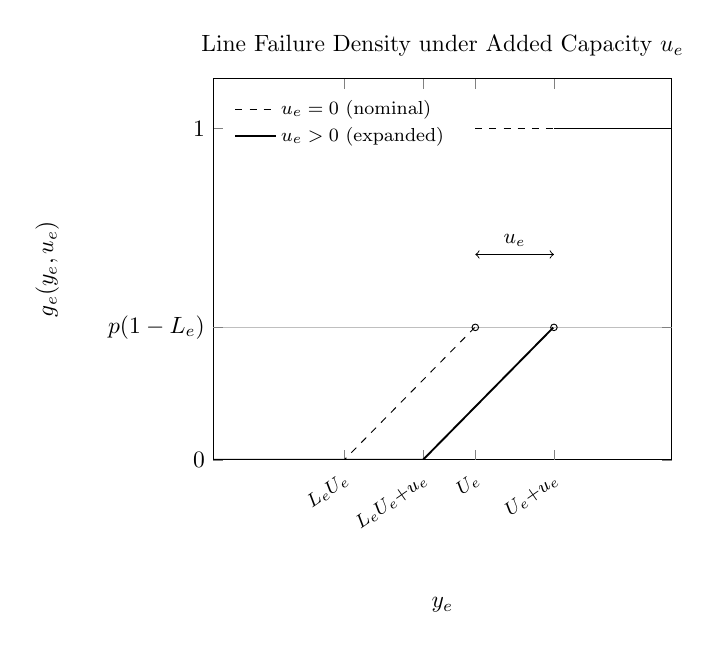
\begin{tikzpicture}[scale=.85]
      \begin{axis}[
	  xlabel=$y_e$,
	  ylabel={$g_e(y_e,u_e)$},
	  title = {Line Failure Density under Added Capacity $u_e$},
	  xtick=\empty,
	  ytick={0,1},
	  extra y ticks={.4},
	  extra y tick style={grid=major},
	  extra y tick labels={$p(1-L_e)$},
	  extra x ticks={.5,.8,1,1.3},
	  extra x tick labels={$L_eU_e$,$L_eU_e{+}u_e$,$U_e$,$U_e{+}u_e$},
	  x tick label style={font=\footnotesize,rotate=35,anchor=north east},
	  xlabel style={yshift=-20pt},
	  ylabel style={yshift=14pt},
	  xmin=0, xmax=1.75,
	  ymin=0, ymax=1.15,
	  legend style={at={(0.03,0.97)},anchor=north west,font=\footnotesize,draw=none,fill=none},
	  legend cell align=left]

	% Nominal system (u_e = 0): rises from L_e U_e, saturates at U_e
	\addplot[black,dashed] coordinates {(0,0) (.5,0) (.9975,.3995)};
	\addlegendentry{$u_e=0$ (nominal)}
	\addplot[black,dashed,forget plot] coordinates {(1,1) (1.75,1)};
	\addplot[black,mark=o,mark size=1.4pt,only marks,forget plot] coordinates {(1,.4)};

	% Expanded system: both the breakpoint and the capacity shift right by u_e
	\addplot[black,thick] coordinates {(0,0) (.8,0) (1.2975,.3995)};
	\addlegendentry{$u_e>0$ (expanded)}
	\addplot[black,thick,forget plot] coordinates {(1.3,1) (1.75,1)};
	\addplot[black,mark=o,mark size=1.4pt,only marks,forget plot] coordinates {(1.3,.4)};

	% The shift induced by the added capacity
	\draw[<->,black] (axis cs:1,.62) -- node[above,font=\small]{$u_e$} (axis cs:1.3,.62);
      \end{axis}
    \end{tikzpicture}

\end{document}
